\documentclass{article}
\usepackage[utf8]{inputenc}
\usepackage[a4paper, portrait, margin=1in]{geometry}
\usepackage{tabularx}
\usepackage{graphicx}
\usepackage{amsmath}
\usepackage{hyperref}
\hypersetup{
    colorlinks=true,
    linkcolor=blue,
    filecolor=magenta,      
    urlcolor=cyan,
}


\title{OOAD \& Software Engineering (UE18CS353) \\
    Unit 3}
\author{Aronya Baksy}
\date{March 2021}

\begin{document}
\maketitle
\section{Design Principles}
\subsection{GRASP}
\begin{itemize}
    \item \textbf{G}eneral \textbf{R}esponsibility \textbf{A}ssignment \textbf{S}oftware \textbf{P}rinciples (or \textbf{P}atterns) is a set of principles that help in assigning responsibilities to objects.
    
    \item Responsibility: a contract/obligation to be fulfilled by a component/class/module
\end{itemize}

\subsubsection{Creator}
\begin{itemize}
    \item Assign $B$ the responsibility of creating object $A$ if:
    \begin{itemize}
        \item Instances of $B$ contain or aggregate instances of $A$
        
        \item Instances of $B$ record instances of $A$
        
        \item Instances of $B$ closely use instances of $A$
        
        \item Instances of$B$ have the initializing information for instances of $A$ and pass it on creation
    \end{itemize}
\end{itemize}

\subsubsection{Information Expert}
\begin{itemize}
    \item Assign those responsibilities to a class which has the information to fulfill that responsibility
    
    \item In case one class does not have all the information, assign the responsibility to the class that has the most information needed to fulfill it. 
\end{itemize}

\subsubsection{Low Coupling}
\begin{itemize}
    \item Coupling is a measure of how inter-dependent objects of 2 different classes are. 
    
    \item Low coupling is always preferred as it minimizes the impact of changes in one class on the dependent classes. 
    
    \item Low coupling makes a system maintainable, efficient and code reusable
    
    \item Two elements are coupled, if :
    \begin{enumerate}
        \item One element has aggregation/composition association with another element.
        
        \item One element implements/extends other element
    \end{enumerate}
\end{itemize}

\subsubsection{Controller}
\begin{itemize}
    \item Minimizing dependency between UI classes and system classes that represent system-level operations.
    
    \item The controller class receives requests from UI layer objects and then controls/coordinates with objects of the domain layer to fulfill the request.
    
    \item The controller can be reused, can maintain the state of the use case and can control the sequence of the activities
\end{itemize}

\subsubsection{High Cohesion}
\begin{itemize}
    \item Merge related responsibilities into single modules. Clearly defining the purpose of a single manageable unit.
    
    \item High cohesion allows for more code reuse, more understandability and maintainability.
\end{itemize}

\subsubsection{Polymorphism}
\begin{itemize}
    \item Responsibility for defining the variation of behaviors \textit{based on type} is assigned to the type for which this variation happens
    
    \item Handle related but varying elements based on their type. 
\end{itemize}

\subsubsection{Pure Fabrication}
\begin{itemize}
    \item A pure fabrication is a class that does not represent any real-world entity, but completes an associated set of responsibilities. 
    
    \item Decomposes the behaviour of a complex class, and thus increases cohesion, reduces coupling and increases reusability.
    
    \item Implemented in Adapter and Strategy design patterns
    
    \item e.g.: A class called DBStore does all database operations and takes that responsibility away from a "Shape" class that does all Shape-related computation
    
    \item e.g.: logInterface which is responsible for logging information 
\end{itemize}
\subsubsection{Indirection}
\begin{itemize}
    \item Avoid direct coupling between 2 classes by introducing an intermediate unit to communicate between the other units, so that the other units are not directly coupled
    
    \item Implemented in Adapter and Fa\c{c}ade design patterns 
\end{itemize}
\subsubsection{Protected Variations}
\begin{itemize}
    \item How to avoid impact of variations of some elements on the other elements
    
    \item Identify points of predicted variation or instability; assign responsibilities to create a stable interface around them
    
    \item Implementation:  Provide an interface so that the there will be no effect on other units and then use polymorphism to create various implementations of this interface
    
    \item  Provides flexibility and more structured design
\end{itemize}

\subsection{SOLID}
\begin{itemize}
    \item Just like GRASP, another set of patterns for implementing best practices/low coupling/high cohesion etc
    
    \item Enables changes, makes code more flexible, maintainable, stable, and reusable
\end{itemize}

\subsubsection{Single Responsiblity Principle}
\begin{itemize}
    \item A class should have only one responsibility
    
    \item This leads to only one reason for changing that class, hence reducing side effects during maintenance
    
    \item The aim of splitting responsibilites is to increase cohesion, minimize coupling.
\end{itemize}

\subsubsection{Open-Closed Principle}
\begin{itemize}
    \item A class should be open for extension but closed for modification. Also stated as: "One should be able to extend the class behavior without modifying it"
    
    \item Implemented using inheritance and composition. In inheritance, the base class behaviour does not need to be touched in order to extend its behaviour using a subclass
\end{itemize}

\subsubsection{Liskov Substitution Principle}
\begin{itemize}
    \item A derived class must be substitutable for its base class
    
    \item Formally, let  $\phi (x)$ be a property provable about objects $x$ of type $T$. Then $\phi(y)$ should be true for objects $y$ of type $S$ where $S$ is a subtype of $T$.
\end{itemize}
\begin{figure}[!h]
    \centering
    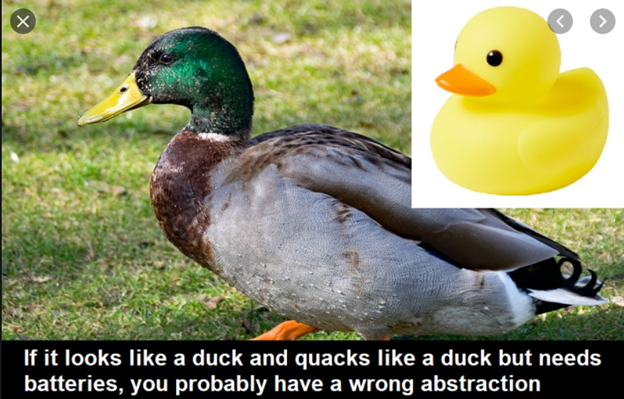
\includegraphics[scale=0.4]{meme.png}
    \caption{Meme about Liskov Substitution}
    \label{fig:my_label}
\end{figure}

\subsubsection{Interface Segregation Principle}
\begin{itemize}
    \item Clients should not be forced to depend upon the interfaces that they do not use.
    
    \item Make fine-grained interfaces that are specific to each client. 
    
    \item Instead of having one interface class that can handle $N$ special cases, it is better to have $N$ interfaces, one for each special case.
\end{itemize}

\subsubsection{Dependency Inversion Principle}
\begin{itemize}
    \item Program to an interface, not to an implementation
    
    \item Formally, it is stated as:
    \begin{itemize}
        \item  High-level modules should not depend on low-level modules. Both should depend on abstractions (e.g., interfaces).
        
        \item Abstractions should not depend on details. Details (concrete implementations) should depend on abstractions.
    \end{itemize}
\end{itemize}

\section{Software Implementation Phase}
\begin{itemize}
    \item The detailed creation of working software through a combination of coding, reviews and unit testing.
    
    \item \textbf{Entry criteria} is design (low-level and high-level, detailed design document) and\textbf{ exit criteria} is unit-tested and peer-reviewed, functioning code. 
    
    \item Involves choice of language, choice of dev env, building and following a config management plan and actual development of code. 
    
    \item Primary goals for implementation phase:
    \begin{itemize}
        \item Minimize complexity
        
        \item Anticipate change
        
        \item Construct readable, testable and reusable code
    \end{itemize}
    
    \item Characteristics of implementation phase:
    \begin{itemize}
        \item Tool dependent: Compiler, debugger, IDE, GUI builders etc.
        
        \item Large volume of config items: source files, test case files, documentation etc.
        
        \item Directly affects software quality
        
        \item Use of CS knowledge: DSA, coding practices etc.
    \end{itemize}
\end{itemize}

\subsection{Primary Considerations}
\begin{itemize}
    \item \textbf{Handling errors}: using exception handling constructions, checking return values, and using assertion statements
    
    \item \textbf{Security breaches}: consider every opportunity for a security breach in the code, e.g. buffer overflow, SQL injection
    
    \item \textbf{Effective use of computation power} on host system, considering other programs also running on that system
    
    \item \textbf{Documentation} about the code, and within the code (combined with machine-readable source code)
    
    \item \textbf{Optmization}: Use performance analysis tools to identify slow-running sections of code, optimize those to run faster
\end{itemize}
\subsection{Choice of programming language}
\begin{itemize}
    \item Assembly languages: operate at the machine level directly (e.g.: ARM assembly, x86\_64 so on)
    
    \item Procedural languages: modest level of abstraction above hardware (e.g. early versions of Fortran/ C/ Pascal)
    
    \item Aspect-oriented languages: Allow more separation of concerns and increase modularity (e.g. basically any language you can think of)
    
    \item Object Oriented: Highest level of abstraction, developers now think of the problem in terms of real-life objects and their behaviour (e.g. C++, Java, C\#, Python, etc.)
\end{itemize}

\subsection{Choice of Development Environment}
\begin{itemize}
    \item Commercial vs Open Source: Developers prefer open source tools (customizable) but enterprises feel that commercial tools are more fully featured
    
    \item Support of process: Availability of extensions that support debugging, static analysis, test building etc.
\end{itemize}

\subsection{Coding Bugs}
\begin{itemize}
    \item Bugs are caught at review or at unit/integration/system testing, acceptance testing or at production
    
    \item The cost of catching a bug at each subsequent stage increases exponentially. Hence catching bugs ASAP is crucial.
\end{itemize}

\subsection{Characteristics of Code}
\begin{itemize}
    \item \textbf{Well structured, well designed}. Not too many lines per function, lines per file, args per function, levels of nesting and conditions
    
    \item \textbf{Meaningful, descriptive but short variable names} that follow consistent naming (Pascal case, camel case or underscore prefix)
    
    \item Restrictions enforced by programming \textbf{language syntax} (keywords, identifier length etc.)
    
    \item Highlight dependencies in software through \textbf{file organization}. Logically grouped and partitioned files, properly initialized data structures (Abstract Data Types or ADTs)
    
    \item \textbf{Easy to read} code with indentation, brackets (when applicable), spaces, newlines, parenthesis for grouping, 
    
    \item \textbf{Well commented} code. Comment should be brief and concise but not cryptic, misleading or redundant.
\end{itemize}

\subsection{Refactoring}
\begin{itemize}
    \item Improve internal structure of code without changing external behaviour
    
    \item Improve non-functional and objective attributes of the code (cyclomatic complexity, length, duplication, coupling/cohesion) that improve understandability and maintenance.
    
    \item Does not involve rewriting code, fixing bugs or changing observable interfaces. 
\end{itemize}

\subsection{Coding Standards and Guidelines}
\begin{itemize}
    \item Standards are mandatory rules, guidelines are just recommendations. Both aim to increase overall code quality.
    
    \item Give an uniform appearance to code that has been written by different people. 
    
    \item Improve readability, maintainability of code by removing effects of different personalities that work on code
\end{itemize}


\subsubsection{Coding Standards}
\begin{itemize}
    \item Promote code reuse, sound practices, and increase efficiency.
    
    \item \textbf{Defensive Programming} is a standard that involves checking for all implicit assumptions and handling each case. Involves adding redundant code that checks system state after each modification 
    
    \item \textbf{Secure Programming} is the practice of developing computer software in a way that guards against the accidental introduction of security vulnerabilities. Practices involved in secure programming are:
    \begin{itemize}
        \item Validate input from untrusted source
        
        \item Heed compiler warnings and eliminate them using analysis tools
        
        \item Default deny all permissions to all modules, unless a permission is absolutely essential for a particular module to function properly. 
        
        \item Principle of least privilege. Each process gets the most minimal set of privileges for the most minimal amount of time that is needed to finish it's work and nothing more
        
        \item Sanitize data sent between external components and your code. 
    \end{itemize}
    
    \item \textbf{Programming for Testability} involves the use of the following:
    \begin{itemize}
        \item \textbf{Assertions} identify out-of-range and inappropriate values
        
        \item \textbf{Test Points} are functions that set and get current module status for debugging
        
        \item \textbf{Scaffolding} emulates the functionality of not-yet-built features for message exchange
        
        \item \textbf{Test harness} is code written to drive incomplete objects/modules as if they were complete
        
        \item \textbf{Test Stub} is a function that returns a fixed value as it has not yet been implemented
        
        \item \textbf{Instrumentation}, aka logging 
        
        \item \textbf{Building test dataset}
    \end{itemize}
 \end{itemize}
 
 \subsubsection{Coding Guidelines}
 \begin{itemize}
     \item Generic suggestions regarding the coding style for betterment of understanding, readability of the code
     
     \item Helps in early error detection that reduces costs
     
     \item Simplifies maintenance
 \end{itemize}
 
 \subsection{Evaluating code quality}
 \subsubsection{Evaluation Metrics}
 \begin{itemize}
     \item Code construction is evaluated from 2 perspectives: progress (in development according to the schedule in the project plan) and quality 
     
     \item Progress and productivity are \textbf{measured} in terms of active days spent, scope completed, code churn etc. \textbf{Metrics} are LoC generated, LoC purged, LoC per effort day
     
     \item Code quality \textbf{measured} in terms of static code analysis results on length, insturction paths, complexity. \textbf{Metric} is number of errors per KLoC
 \end{itemize}
 
 \subsubsection{Special Evaluation Metrics for Agile projects}
 \begin{itemize}
     \item \textbf{Sprint Breakdown} is a chart wherein time is plotted on the x axis and the work remaining (in terms of number of user stories) is plotted on the y axis. The expected and actual progress can be measured and compared using such a chart 
     
     \item \textbf{Team Velocity} measures the number of stories the team completes per sprint. It can be measured in story points or hours, and can be used for estimation and planning.
     
     \item \textbf{Throughput} is the total value added work per unit time. Measured as number of tickets (i.e. stories) completed per unit time. 
     
     \item \textbf{Cycle Time} is the time elapsed between a team starting work on an item and completing that work. 
 \end{itemize}


\subsubsection{Ensuring code quality: Review}
\begin{itemize}
    \item \textbf{Peer Review}: informal advice given by other developers about the code
    
    \item \textbf{Unit Test}: write code that calls functions and checks their correct functionality
    
    \item \textbf{Test-first}: First build test harness, then write code. Ensures that developers don't cheat by writing tests that pass on their code only
    
    \item \textbf{Code Stepping}: Execute code line by line and check system state (variable values etc.) at each time to check control flow.
    
    \item \textbf{Pair Programming}: Two developers, one focusing on function logic, another one on syntax and accuracy
    
    \item \textbf{Code Inspection}: formal review of code in front of a review board that consists of code inspectors
\end{itemize}

\subsubsection{Code Inspection}
\begin{itemize}
    \item Build checklist:
    \begin{itemize}
        \item Based on common errors, past experience
        
        \item Checklists are language dependent and reflect the most common errors that are likely to occur in that language
        
        \item In general, the 'weaker' the type checking, the larger the checklist.
        
        \item e.g.: Initialization, Constant naming, loop termination, array bounds, etc.
    \end{itemize}
    
    \item Planning: Select team, venue. Make documentation and code available to inspection team in advance.
    
    \item Inspection takes place, errors are noted, modifications are made if necessary to repair those errors. 
    
    \item Re-inspection may or may not be required post the changes
    
    \item All of these are documented and archived
\end{itemize}

\subsubsection{Unit Testing Tools}
\begin{itemize}
    \item \textbf{Unit-Testing Frameworks}: Enter method to be tested, arguments, and expected output. Framework automates the method call, test and reporting process. (e.g.: Nunit for .NET apps, Junit for Java apps)
    
    \item \textbf{Coverage Analyzers and Debuggers}: Find percentage of code that is covered by unit tests, and locate and fix errors (e.g.: JaCoCo available with Eclipse for Java apps, Cobertura, PureCoverage)
    
    \item \textbf{Wizards}: automated test generation given input parameters 
    
    \item \textbf{Record-Playback Tools}: Start a session, record a sequence of mouse and keyboard activities and replay those later quickly and accurately (e.g.: Selenium)
\end{itemize}

\section{Software Configuration Management (SCM)}
\begin{itemize}
    \item A process for systematic organization, management and control of entities generated during each phase of the SE process for the product under consideration
    
    \item Increase productivity, increase and plan coordination among the programmers in a team and eliminate confusion
    
    \item In a Scrum team, SCM is the responsibility of the entire team. Max amount of automation is used for SCM process. 
    
    \item In a Scrum team, evelopers pull from central repo. Make changes in their local env, perform unit tests, once the tests all pass then push changes to central repo. 
\end{itemize}

\subsection{Benefits of SCM}
\begin{itemize}
    \item Permit orderly development, as well as orderly implementation and release of software items. 
    
    \item Only approved changes (ones that conform to specification) are deployed. No unauthorized changes are added to the central repo. 
    
    \item Keeps documentation updated to reflect changes. Communicate changes and their impact to all stakeholderss
\end{itemize}

\subsection{Roles in SCM}
\begin{itemize}
    \item \textbf{Configuration Manager}: Identify config items, identify procedures for promotion and release
    
    \item \textbf{CCB Member}: Approve/reject change requests
    
    \item \textbf{Developer}: Implement versions based on project plan or change request. Check changes, resolve conflict
    
    \item \textbf{Auditor}: review the selection process for promotions for release. Ensure completeness and consistency of release
\end{itemize}

\subsection{Config Management Plan}
\begin{itemize}
    \item This is the outcome of the SCM Planning phase. Done by the config manager in a full time or part time capacity. 
    
    \item Can be made company-specific or according to some template like IEEE 828
    
    \item SCM Plan normally contains the following:
    \begin{itemize}
        \item Config Items (CIs) to be managed, and naming scheme for the same
        
        \item Who is responsible for config management and baseline creation
        
        \item Change control and version control policies
        
        \item Tools to assist in config management. Limitations of those tools
        
        \item Config management database used to record info during the SCM process
    \end{itemize}
\end{itemize}

\subsection{Activities in SCM}
\subsubsection{CI Identification}
\begin{itemize}
    \item A config item (CI) is an entity (software or hardware or aggregation of the two) that is designated for SCM 
    
    \item e.g.: code files, test drivers, documentation, manuals, software/hardware config, 
    
    \item Selection of CI similar to class modelling. Identify entites and their relationships. 
    
    \item Starting SCM too early leads to bureaucratic complications. Starting SCM too late leads to chaos.
\end{itemize}

\subsubsection{CM Directories}
\begin{itemize}
    \item The \textbf{programmer's directory} is controlled by the developer only. It contains newly created or modified CIs only
    
    \item The \textbf{master directory} is an entry-controlled, authorized directory used for managing current baselines and controlling changes made to those baselines. 
    
    \item The \textbf{software repository} is an archive for the various baselines released to the public. These are distributed to requesting parties 
\end{itemize}

\subsubsection{Baseline}
\begin{itemize}
    \item A specification or product that has been formally reviewed and agreed to by responsible management, that serves as the basis for further development, and can only be changed through formal change control procedures
    
    \item Baselines may or may not be tied to the schedule defined in the project plan. 
\end{itemize}

\subsubsection{Branch Management}
\begin{itemize}
    \item A branch is a copy of the source code (fully or a part) within the repository. Branching is done for the following reasons:
    \begin{itemize}
        \item Support concurrent development
        
        \item Support multiple versions of a solution
        
        \item Enables experimentation by developers without affecting the central codebase
    \end{itemize}
    
    \item Merging is bringing back and integrating the changes done in branches to the working branch. Frequent merging from related branches into the working branch helps decreasing the likelihood and complexity of a merge conflict
        
    \item Branch strategies:
    \begin{itemize}
        \item Single working branch
            
        \item Branch by developer or workspace
            
        \item Branch by customer or organization
        
        \item Branch by module or component
    \end{itemize}
\end{itemize}

\subsubsection{Version Management}
\begin{itemize}
    \item Tracking different versions of components used in a software project
    
    \item Typically tools like Git are used for this purpose.
    
    \item Features of version control:
    \begin{itemize}
        \item All versions are identified by a unique version number
        
        \item All changes are traceable
        
        \item Change history is recorded to allow rollback of changes if needed
        
        \item Conflict resolution, maintenance and quality monitoring. 
        
        \item Less software regression 
    \end{itemize}
\end{itemize}

\subsubsection{Build Management}
\begin{itemize}
    \item Compiling all source code files and libraries, and linking them together to build an executable program or a binary. 
    
    \item Build utilities compile the files in the correct logical order (in case there are no changes to a file it may not be compiled again) and then links the generated binaries together
    
    \item Build automation tools like Maven, make (the GNU standard tool), Apache Ant
    
    \item Build Process:
    \begin{enumerate}
        \item Fetch code from source control repo
        
        \item Compile the code. Check dependencies and then link the libraries and code appropriately
        
        \item Run unit tests (manual or automated)
        
        \item Once all tests pass, build the artefact and store them. Archive the generated build logs. 
        
        \item Notify all stakeholders, then update the version number
    \end{enumerate}
    
    \item A build can either be a \textbf{full build} (from scratch, all files) or an \textbf{incremental build} (only changed files are recompiled and linked)
    
    \item Build process can be triggered by:
    \begin{itemize}
        \item Manual trigger
        
        \item Scheduled trigger
        
        \item Repository trigger 
        
        \item Post process build trigger
    \end{itemize}
\end{itemize}

\subsubsection{Install Management}
\begin{itemize}
    \item Involves placing multiple executable files, downloading or copying from a repository. 
    
    \item Could also involve downloading executable files, config files, libraries, images etc. from the internet
    
    \item Also involves interaction with the OS when requesting for resources to run the software, and managing appropriate permissions. 
    
    \item Automated install management is performed by tools like InstallShield, InstallAware, Jenkins etc.
\end{itemize}

\subsubsection{Change Management}
\begin{itemize}
    \item General process of change management:
    \begin{itemize}
        \item Change is requested. This change request is logged into a tool along with some metadata about the change (change ID, date, who raised, etc.)
        
        \item The cost and overall development impact of the change is assessed. The result of this assessment is either the change request being accepted or rejected
        
        \item If accepted then the change is implemented, validated and audited
        
        \item The documentation is updated. Plans made for versioning, merging, delivery are followed.
    \end{itemize}
    
    \item Smaller projects have simple and informal change management. Larger projects have a change control board (CCB) that documents all changes and accepts/rejects requests
    
    \item A change is described by its description, reason for making the change and other items affected by this change. 
    
    \item Change management is highly automated and tool driven. Change logging tools like Jira, file comparision tools for tracking changes, etc. 
    
    \item Change control policies: 
    \begin{itemize}
    
        \item Change policies guarantee that each version, revision or release conforms to commonly accepted criteria and ensures consistent process throughout.

        \item These change policies are enforced through engineering processes and tools. They are also audited to ensure they conform to the processes defined
    \end{itemize}
\end{itemize}

\subsubsection{Promotion Management}
\begin{itemize}
    \item Policies that control the pushing of code from programmer directory to the master directory. 
    
    \item Policies are based on baselining criteria, and include validation, followed by a process of verification and authorization of the changes made. 
    
    \item e.g. for promotion policy: "No developer is allowed to promote source code which cannot be compiled without errors and warnings"
\end{itemize}

\subsubsection{Release Management}
\begin{itemize}
    \item Policies that control movement of code from master directory to the software repository, and its release to the final customer. 
    
    \item The policy is based on:
    \begin{itemize}
        \item Quality criteria, verification of metrics for the same
        
        \item If quality criteria are met, release is authorized and code is archived to the software repository
    \end{itemize}
    
    \item e.g. for release policy: "No baseline can be released without having been beta-tested by at least 500 external persons"
    
    \item A \textbf{patch} is a set of updates made to a code to improve, update or fix any issues in it. 
    
    \item A service pack or SP or a feature pack (FP) comprises a collection of updates, fixes, or enhancements to a software program delivered in the form of a single package.
    
    \item Patches can be generic, hot patches, source code/binary patches, or emergency patches.
\end{itemize}

\subsubsection{Defect Management}
\begin{itemize}
    \item Defect is a variation between the actual behaviour of the software product and the expected business requirements. 
    
    \item Bugs are tracked and fixed using automated tools like BugZilla
    
    \item Steps in defect management:
    \begin{enumerate}
        \item Discover bug. Report it and log it into a tool with an unique ID
        
        \item Validation, analysis, priority (critical, high, med, low)
        
        \item Open formal request and get approval for the same. 
        
        \item Bug resolution (assignment, schedule, fix, test, report)
        
        \item Verification by submitter of bug report. Once verified merge code
        
        \item Update version number, plan release of the bug fix.
        
        \item Close the process, generate report. 
    \end{enumerate}
\end{itemize}
\end{document}